% CVPR 2026 Paper Template

\documentclass[10pt,twocolumn,letterpaper]{article}

%%%%%%%%% PAPER TYPE
% \usepackage[review]{cvpr}
\usepackage[pagenumbers]{cvpr}

\input{preamble}

\definecolor{cvprblue}{rgb}{0.21,0.49,0.74}
\usepackage[pagebackref,breaklinks,colorlinks,allcolors=cvprblue]{hyperref}

\def\paperID{*****}
\def\confName{CVPR}
\def\confYear{2026}

\title{Domain-Specific 3D Gaussian Splat Generation: Fine-Tuning DiffSplat for Anime Characters}

\author{
Jianpeng Li \qquad Ruolan Chen \qquad Jianxiang Ling\\
Cornell University\\
{\tt\small \{jl4646, rc975, jl4647\}@cornell.edu}
}

\begin{document}
\maketitle

\begin{abstract}
Generating high-quality 3D character assets remains difficult for small teams because it usually requires significant manual modeling expertise. This problem is especially challenging for anime characters, whose visual identity depends on stylized geometry, sharp color separation, expressive hair shapes, flat shading, and non-photorealistic outlines. In this project, we explore whether DiffSplat, a diffusion-based framework for generating 3D Gaussian Splats, can be adapted to this stylized domain through small-scale fine-tuning. We build a Blender-based data preparation pipeline that renders multi-view images from anime character models and converts them into a training format for DiffSplat fine-tuning. Our dataset contains 20 unique anime characters with 40 rendered views per character. We evaluate the fine-tuned model using both qualitative multi-view renderings and quantitative image metrics. Our results show that direct fine-tuning can partially adapt the model to anime-style inputs, but it still struggles with washed-out textures, collapsed character details, and inconsistent geometry. These findings suggest that the main challenge is not only the 2D image prior, but also the object-centric bias and weak geometric supervision of the original 3D generation pipeline.
\end{abstract}

\section{Introduction}

High-quality 3D character creation is expensive and time-consuming. A production-ready character often requires manual modeling, UV unwrapping, texturing, rigging, and repeated artist revision. This creates a large gap between people who can design 2D characters and people who can build usable 3D assets. The gap is even more visible in anime and game-style characters, where the model must preserve highly recognizable visual details such as hair silhouettes, clothing shapes, facial proportions, and strong color blocks.

Recent generative models have made major progress in 2D image generation and 3D asset generation. Latent diffusion models show that pretrained image diffusion backbones can provide strong visual priors for high-quality image synthesis~\cite{rombach2022ldm}. 3D Gaussian Splatting represents scenes using anisotropic Gaussians and enables efficient real-time rendering~\cite{kerbl20233dgs}. DiffSplat builds on these ideas by adapting pretrained image diffusion models to generate 3D Gaussian Splats directly, supporting both text-conditioned and single-image-conditioned 3D generation~\cite{lin2025diffsplat}. This makes DiffSplat a promising starting point for our task, because our target use case is generating a 3D character representation from a single anime character image.

However, most existing 3D generation systems are still stronger on photorealistic objects than on stylized human-like characters. Anime characters are not simply ``objects with different textures.'' They often contain thin limbs, exaggerated hair, flat regions of color, non-realistic outlines, and clothing folds that do not follow ordinary object geometry. These properties make the domain a useful stress test for current 3D generative models.

In this project, we investigate the following question: can a pretrained DiffSplat model be fine-tuned into a domain-specific anime character generator using a small multi-view dataset? Our contributions are:
\begin{enumerate}
    \item We build an automated Blender-to-dataset pipeline for rendering anime character models from multiple views.
    \item We fine-tune DiffSplat on a small stylized character dataset with 20 characters and 40 views per character.
    \item We analyze the main failure modes of direct fine-tuning for anime characters, including texture wash-out, feature collapse, and broken multi-view structure.
    \item We discuss why small-scale fine-tuning is insufficient and propose future directions based on better stylized datasets and geometric guidance.
\end{enumerate}

\section{Method}

\subsection{Task Definition}

Given a single input image of an anime character, our goal is to generate a 3D Gaussian Splat representation that can be rendered from novel viewpoints. The desired output should preserve both character identity and 3D consistency. In practice, this means the generated model should maintain recognizable hair shape, clothing structure, color separation, body proportions, and stable appearance across camera views.

We use DiffSplat as the base model because it directly generates 3D Gaussian Splats while reusing the visual prior of a pretrained 2D diffusion model. Compared with training a 3D-native model from scratch, fine-tuning DiffSplat is more practical for a course project because the model already contains strong image-level knowledge and supports single-image conditioning.

\subsection{DiffSplat Background}

DiffSplat can be understood as a pipeline that maps an input condition to a latent 3D representation and then decodes it into Gaussian Splats. The generated Gaussian representation can be rendered from novel views. Unlike a pure 2D image diffusion model, DiffSplat uses 3D-aware components to maintain consistency across viewpoints. This is important for our project because a successful anime character generator should not only produce a good front-view image, but also preserve the character when viewed from the side or back.

\begin{figure}
    \centering
    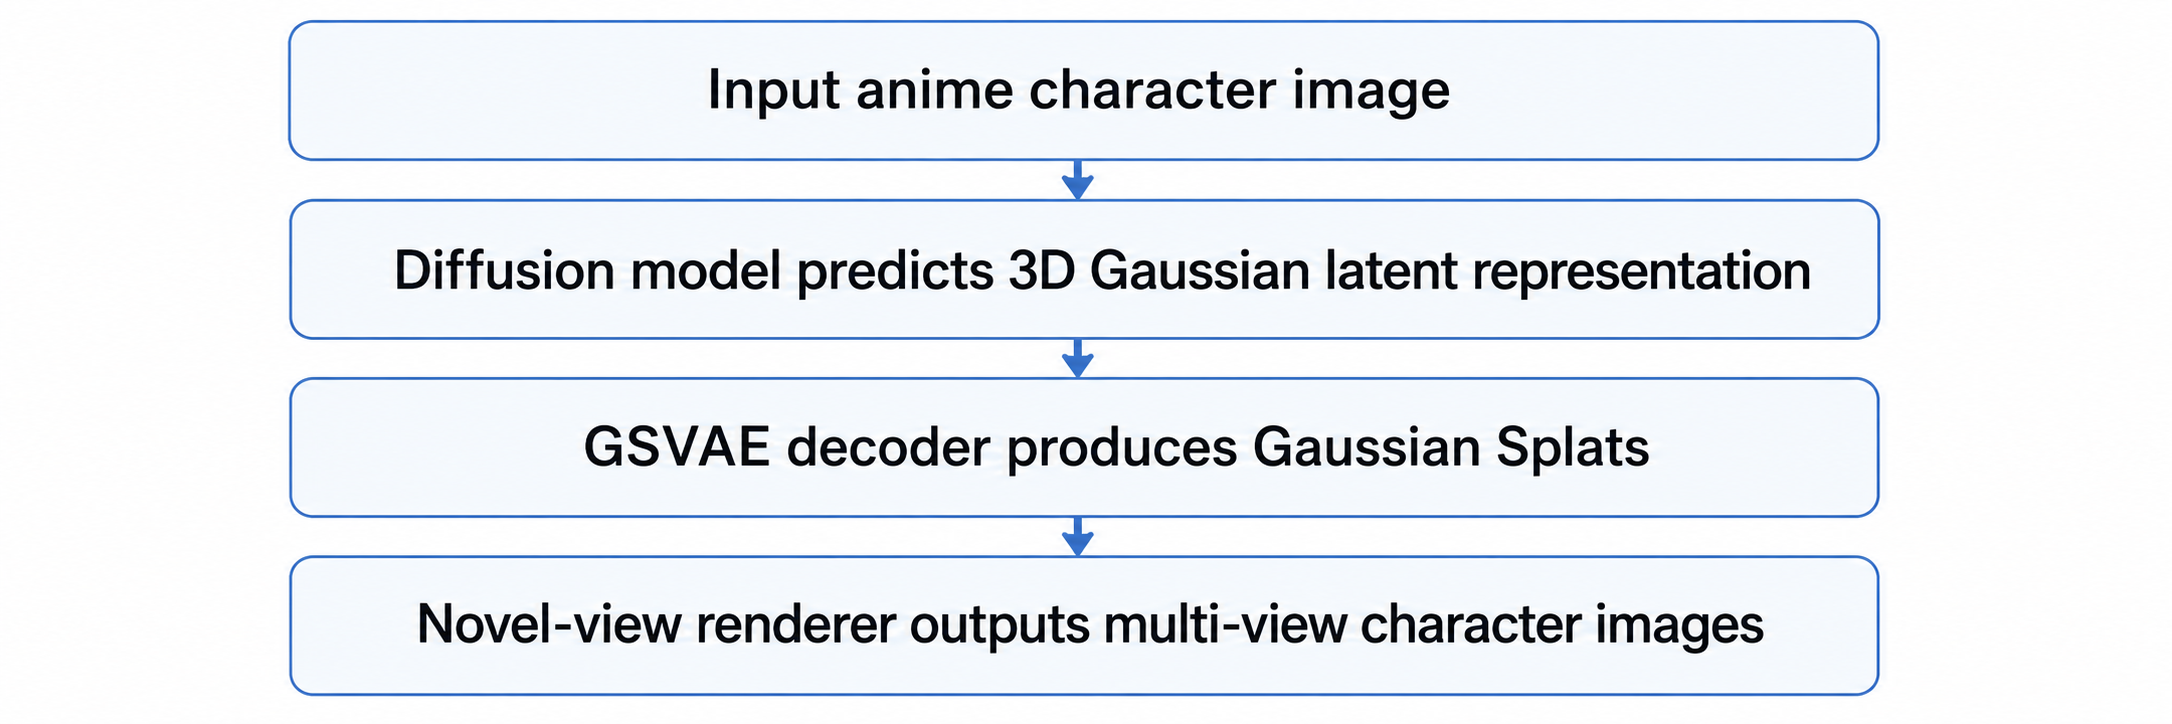
\includegraphics[width=0.9\linewidth]{image.png}
    \caption{Overview of our fine-tuning pipeline. We adapt DiffSplat to the anime character domain by preparing multi-view renderings from stylized 3D models and using them to fine-tune the Gaussian Splat generation model. Replace this placeholder with your actual method figure if available.}
    \label{fig:method}
\end{figure}



\subsection{Data Preparation}

A central part of our project is the data preparation pipeline. We collect anime-style 3D character models and use Blender to render them from multiple camera angles. For each character, we generate 40 views with controlled camera poses. This gives the model view-dependent supervision and helps it learn how stylized character features should appear across different angles.

Our final dataset contains 20 unique anime characters. For each character, the pipeline performs the following steps:
\begin{enumerate}
    \item load the character model in Blender;
    \item normalize the character scale and camera position;
    \item render 40 images around the character;
    \item save camera and rendering metadata;
    \item pack the rendered images into the format required by the DiffSplat fine-tuning code.
\end{enumerate}

This automated pipeline is important because manually preparing multi-view data would be slow and error-prone. It also makes the project easier to extend: adding more characters only requires placing new models into the input directory and running the rendering script again.

\subsection{Fine-Tuning Setup}

We fine-tune the DiffSplat model on our anime character dataset. Our goal is not to train a new model from scratch, but to test whether the pretrained model can shift toward the anime character domain with limited data. During fine-tuning, the model observes multi-view renderings of the same character and learns to predict a 3D Gaussian representation that can explain these views.

Because our dataset is small, we treat this experiment as a domain adaptation study rather than a full production-quality training run. The fine-tuned model is compared against the original pretrained DiffSplat model. This comparison helps us separate two questions: whether DiffSplat already has some ability to generate stylized characters, and whether our fine-tuning improves or worsens this ability.

\section{Experiments}

\subsection{Dataset}

We use a custom anime character dataset created through our Blender rendering pipeline. The dataset contains 20 unique characters and 40 views per character, resulting in 800 rendered training images. The characters include human-like bodies, stylized hair, clothing, and accessories. These features make the dataset more challenging than simple rigid objects because many important details are thin, non-symmetric, or highly stylized.

We split the rendered views into training and validation views. Training views are used for fine-tuning, while held-out views are used to check whether the model can preserve appearance under novel viewpoints. Since our dataset is small, the validation results should be interpreted as an early diagnostic rather than a complete benchmark.

\subsection{Baselines}

We compare our fine-tuned model against the original pretrained DiffSplat model. The baseline receives the same type of input image but does not receive anime-domain fine-tuning. This is a natural baseline because our main research question is whether domain-specific fine-tuning helps.

We also use the input multi-view renderings as an upper-bound reference for visual quality. These renderings are not a generated baseline, but they show what the character should look like when geometry and texture are correct.

\subsection{Evaluation Metrics}

We use both qualitative and quantitative evaluation. Qualitative evaluation is important because anime character quality is strongly related to visual identity. A model can obtain reasonable pixel-level scores while still failing to preserve recognizable character features. Therefore, we inspect rendered outputs from multiple views and focus on:
\begin{itemize}
    \item color separation and texture clarity;
    \item preservation of hair, face, clothing, and accessories;
    \item consistency between front, side, and back views;
    \item structural coherence of limbs and silhouette.
\end{itemize}

For quantitative evaluation, we use PSNR and LPIPS on held-out validation views. 
PSNR measures pixel-level reconstruction quality and is defined as
\begin{equation}
\mathrm{PSNR}(I, \hat{I}) = 10 \log_{10} \left(\frac{MAX_I^2}{\mathrm{MSE}(I, \hat{I})}\right),
\end{equation}
where $I$ is the ground-truth rendered view, $\hat{I}$ is the generated view, and $MAX_I$ is the maximum possible pixel value. Higher PSNR indicates better pixel-level similarity.

LPIPS measures perceptual similarity using deep feature representations:
\begin{equation}
\mathrm{LPIPS}(I, \hat{I}) = \sum_l w_l \left\| \phi_l(I) - \phi_l(\hat{I}) \right\|_2^2,
\end{equation}
where $\phi_l(\cdot)$ denotes features extracted from layer $l$ of a pretrained network and $w_l$ is a learned layer weight. Lower LPIPS indicates stronger perceptual similarity.

\begin{table}[t]
\centering
\begin{tabular}{lcc}
\hline
Model & PSNR $\uparrow$ & LPIPS $\downarrow$ \\
\hline
Pretrained DiffSplat & XX.XX & X.XXX \\
Fine-tuned DiffSplat & XX.XX & X.XXX \\
\hline
\end{tabular}
\caption{Quantitative comparison on held-out anime character views. Replace the placeholder values with your final results from the notebook.}
\label{tab:quant}
\end{table}

\subsection{Qualitative Results}

Our initial results reveal a clear domain gap. The pretrained DiffSplat model works better on photorealistic or object-like inputs, but anime characters expose several failure modes. After fine-tuning, the output becomes somewhat more aligned with the anime domain, but the improvement is limited.

The most common problem is muddy and washed-out texture. Anime characters often rely on sharp color boundaries, but the generated results tend to blend colors together. This makes clothing, hair, and accessories less readable. Another problem is feature collapse. Thin and distinctive details such as hair spikes, headbands, hats, and small clothing parts often become blurred or disappear. The third problem is broken structural coherence. From some viewpoints, the body silhouette becomes unstable, and the generated result no longer looks like a consistent 3D character.

\begin{figure}[t]
    \centering
    \fbox{
    \begin{minipage}{0.92\linewidth}
    \centering
    \vspace{20pt}
    Insert qualitative comparison here:\\
    input image / baseline views / fine-tuned views / ground-truth rendered views
    \vspace{20pt}
    \end{minipage}
    }
    \caption{Qualitative results. The fine-tuned model partially adapts to anime-style inputs, but still shows washed-out textures, missing stylized details, and inconsistent multi-view structure. Replace this placeholder with your actual generated images.}
    \label{fig:qual}
\end{figure}

\subsection{Analysis}

Our experiments suggest that the main difficulty is not only limited training time or imperfect hyperparameters. Anime characters differ from the original training distribution in several important ways.

First, anime rendering provides weaker physical cues than natural images. Flat shading and outline-based drawing reduce the lighting and material signals that a 3D model may rely on to infer shape. Second, characters are geometrically more complex than many rigid objects. Hair, cloth, limbs, and accessories create thin structures that are easy to blur or merge. Third, small-scale fine-tuning may not be enough to overcome the object-centric bias of the pretrained 3D generation pipeline. Even if the 2D diffusion prior understands anime images, the 3D generation module may still struggle to convert those stylized cues into stable Gaussian geometry.

These results show that direct fine-tuning is a useful first step, but it is not sufficient for high-quality anime character generation. A stronger solution would likely require more data, cleaner annotations, and explicit geometric guidance.

\section{Conclusion}

We explored domain-specific 3D Gaussian Splat generation by fine-tuning DiffSplat on anime characters. We built an automated Blender-to-dataset pipeline, rendered 20 anime characters from 40 views each, and used this dataset to test whether small-scale fine-tuning can adapt a pretrained 3D generative model to a stylized domain.

Our results show that DiffSplat is a promising starting point because it supports single-image conditioning and efficient Gaussian Splat rendering. However, anime characters remain challenging. The generated outputs often show washed-out colors, missing fine details, and inconsistent geometry across views. The key takeaway is that stylized character generation requires more than a generic 2D prior: it also needs stronger 3D structural supervision and a dataset that better captures anime-specific geometry.

For future work, we would first curate a larger and cleaner multi-view anime character dataset with more consistent topology and metadata. We would also add geometric guidance, such as depth maps, normal maps, silhouettes, or ControlNet-style conditioning, to provide stronger structural constraints during generation. These changes may help the model preserve character identity while maintaining coherent 3D structure.

{
\small
\bibliographystyle{ieeenat_fullname}
\bibliography{main}
}

\end{document}